\documentclass[t, final, 12pt, xcolor={usenames,dvipsnames}, table]{beamer}

\usepackage{xcolor}
\usepackage{listings}
%\usepackage{lstlinebgrd}
\usepackage[normalem]{ulem}
\useunder{\uline}{\ul}{}


 
\definecolor{codegreen}{rgb}{0,0.6,0}
\definecolor{codegray}{rgb}{0.5,0.5,0.5}
\definecolor{codepurple}{rgb}{0.58,0,0.82}
\definecolor{backcolour}{rgb}{0.95,0.95,0.92}

\lstset{
    basicstyle=\scriptsize\ttfamily,
    keywordstyle=\color{blue},
    identifierstyle=\color{black},
    commentstyle=\color{orange},
	stringstyle=\color{codepurple},
    showstringspaces=false,
    numberstyle=\color{gray}\tiny,
    breakatwhitespace=false,         
    breaklines=true,                 
    captionpos=b,                    
    keepspaces=true,                 
    numbers=left,                    
    numbersep=5pt,                  
    showspaces=false,                
    showstringspaces=false,
    showtabs=false,                  
    tabsize=2,
    extendedchars=\true,
    inputencoding=utf8,
    frame=tb, 
    columns=fixed,
    backgroundcolor=\color{red!32!green!33!blue!5},
    language=Python
}

\usetheme[pageofpages=of,
          alternativetitlepage=true,
          titlepagelogo=python-logo-big,
          ]{Torino}
          
\usecolortheme{freewilly}


\author{Luiz Alberto}
\title{Python para Ciência de Dados}
\subtitle{Matplotlib Básico}
\institute{Ciência da Computação}
\date{\today}

\logo{
\includegraphics[height=0.125\paperheight]{python-logo-small}}

\begin{document}
  
  \begin{frame}[t,plain]
    \titlepage
  \end{frame}
  
  
  \begin{frame}[t, fragile]{Matplotlib}
  \begin{block}{Definição:}
    Biblioteca python para plotagem de gráficos 2D (incluindo 3D)   (\url{www.matplotlib.org}). 
  \end{block}
  \begin{itemize}
    \item Simplicidade de utilização
    \item Desenvolvimento gradual e interativo
    \item Grande controle sobre os elementos gráficos
    \item Exportação em formatos PNG, PDF, SVG e EPS 
  \end{itemize}
\end{frame}
%
\begin{frame}[t, fragile]{Vizualização de Dados}
  \begin{itemize}
    \item Muito importante na visualização de dados
    \begin{itemize}
      \item Explorar os dados
      \item Apresentar "insights"
    \end{itemize}
  \end{itemize}
  \begin{figure}
    
\includegraphics[scale=.30]{aula-2/figuras/matplot-dataviz-a.jpg}
  \end{figure}
\end{frame}
%

 
  \begin{frame}[t, fragile]{Line plot}
  \begin{columns}
    \begin{column}{0.5\textwidth}
        \lstinputlisting[language=python]{aula-2/codigos/matplotlib/matplotlib-lineplot-1.py}  
    \end{column}

    \begin{column}{0.5\textwidth}
      \begin{center}
        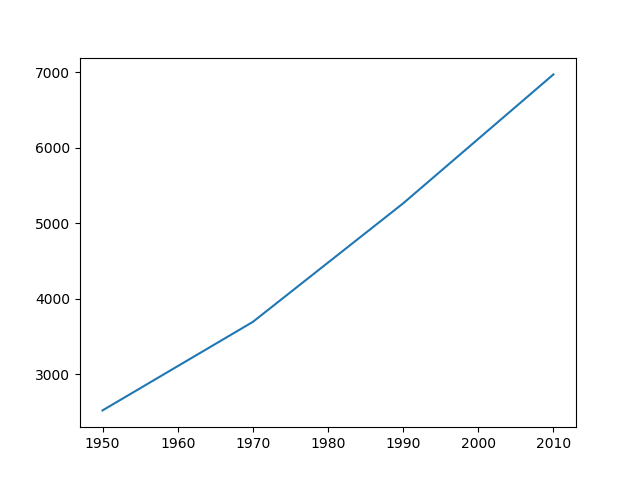
\includegraphics[scale=.40]{aula-2/figuras/matplotlib-lineplot-1.png}
      \end{center}
    \end{column}
  \end{columns}
\end{frame}
%

 
  \begin{frame}[t, fragile]{Scatter plot}
  \begin{columns}
    \begin{column}{0.5\textwidth}
        \lstinputlisting[language=python]{aula-2/codigos/matplotlib/matplotlib-scatterplot-1.py}  
    \end{column}

    \begin{column}{0.5\textwidth}
      \begin{center}
        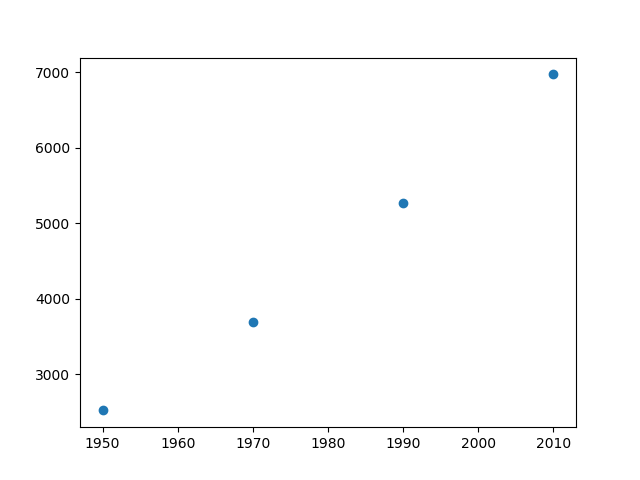
\includegraphics[scale=.40]{aula-2/figuras/matplotlib-scatterplot-1.png}
      \end{center}
    \end{column}
  \end{columns}
\end{frame}
%

 
  \begin{frame}[t, fragile, allowframebreaks]{Hora de colocar a mão na massa}
  Salvar cada um dos exercícios a seguir em um arquivo separado.
\end{frame}
  \begin{frame}[t, fragile]{Histogram}
  \begin{itemize}
    \item Utilizado para explorar dados
    \item Fornece uma idea da distribuição dos dados
  \end{itemize}
  \begin{figure}
    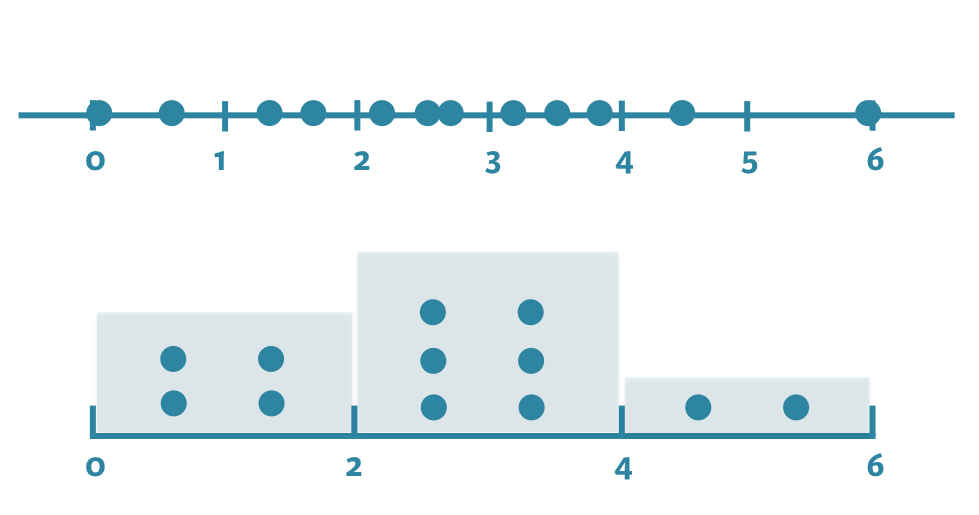
\includegraphics[scale=.40]{aula-2/figuras/matplotlib-histogram-a.png}
  \end{figure}

\end{frame}
%
\begin{frame}[t, fragile]{Histogram}
  \begin{columns}
    \begin{column}{0.5\textwidth}
        \lstinputlisting[language=python]{aula-2/codigos/matplotlib/matplotlib-histogram-1.py}  
    \end{column}

    \begin{column}{0.5\textwidth}
      \begin{center}
        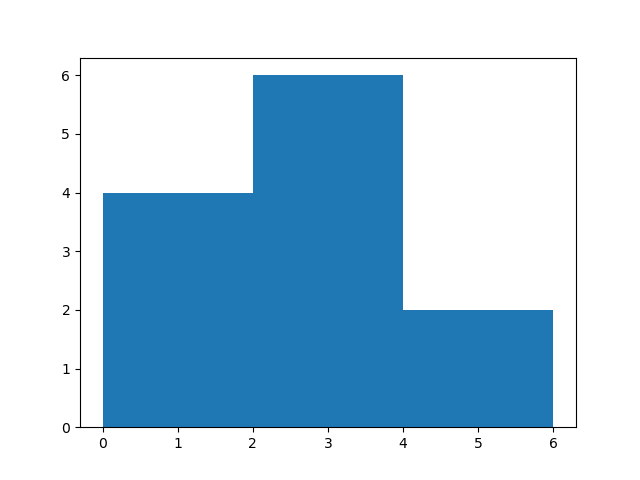
\includegraphics[scale=.40]{aula-2/figuras/matplotlib-histogram-1.png}
      \end{center}
    \end{column}
  \end{columns}
\end{frame}
%

 
  \begin{frame}[t, fragile]{Customização}
  \begin{itemize}
    \item Existem muitas opções
    \begin{itemize}
      \item Diferentes tipos de gráficos
      \item Diversas customizações
    \end{itemize}
    \item A escolha depende
    \begin{itemize}
      \item Dados
      \item Estória a ser contada
    \end{itemize}
  \end{itemize}
\end{frame}
%
\begin{frame}[t, fragile]{Customização}
  \begin{columns}
    \begin{column}{0.55\textwidth}
        \lstinputlisting[language=python]{aula-2/codigos/matplotlib/matplotlib-customization-1.py}  
    \end{column}

    \begin{column}{0.45\textwidth}
      \begin{center}
        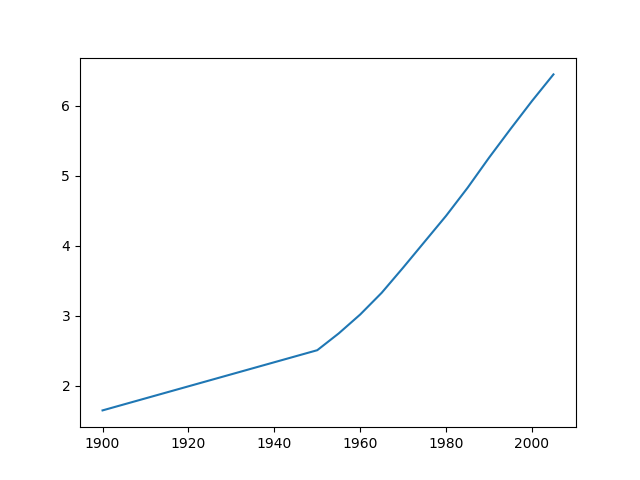
\includegraphics[scale=.35]{aula-2/figuras/matplotlib-customization-1.png}
      \end{center}
    \end{column}
  \end{columns}
\end{frame}
%
\begin{frame}[t, fragile]{Títulos dos eixos X e Y}
  \begin{columns}
    \begin{column}{0.55\textwidth}
        \lstinputlisting[language=python]{aula-2/codigos/matplotlib/matplotlib-customization-2.py}  
    \end{column}

    \begin{column}{0.45\textwidth}
      \begin{center}
        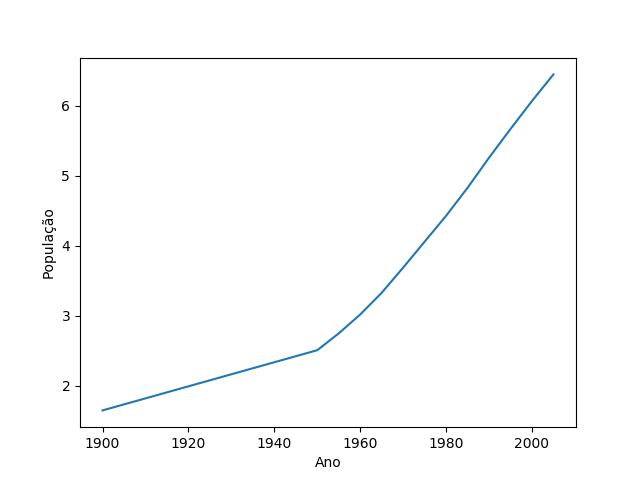
\includegraphics[scale=.35]{aula-2/figuras/matplotlib-customization-2.png}
      \end{center}
    \end{column}
  \end{columns}
\end{frame}
%
\begin{frame}[t, fragile]{Título Principal}
  \begin{columns}
    \begin{column}{0.55\textwidth}
        \lstinputlisting[language=python, firstline=12]{aula-2/codigos/matplotlib/matplotlib-customization-3.py}  
    \end{column}

    \begin{column}{0.45\textwidth}
      \begin{center}
        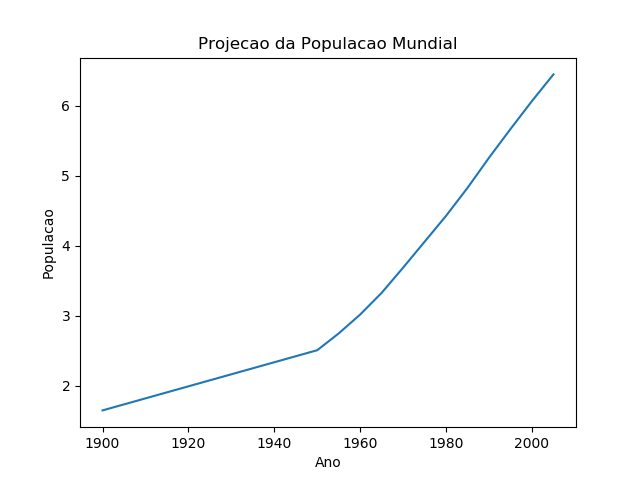
\includegraphics[scale=.35]{aula-2/figuras/matplotlib-customization-3.png}
      \end{center}
    \end{column}
  \end{columns}
\end{frame}
%
\begin{frame}[t, fragile, allowframebreaks]{Ticks}
  \begin{columns}
    \begin{column}{0.55\textwidth}
        \lstinputlisting[language=python, firstline=12]{aula-2/codigos/matplotlib/matplotlib-customization-4.py}  
    \end{column}

    \begin{column}{0.45\textwidth}
      \begin{center}
        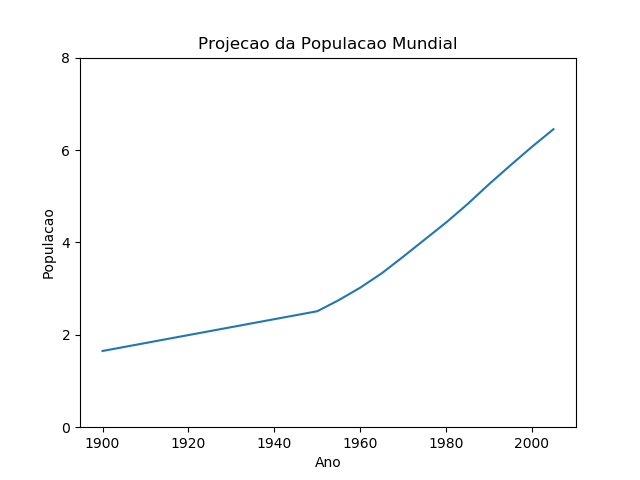
\includegraphics[scale=.35]{aula-2/figuras/matplotlib-customization-4.png}
      \end{center}
    \end{column}
  \end{columns}
  
  \framebreak
  
  \begin{columns}
    \begin{column}{0.55\textwidth}
        \lstinputlisting[language=python, firstline=12]{aula-2/codigos/matplotlib/matplotlib-customization-5.py}  
    \end{column}

    \begin{column}{0.45\textwidth}
      \begin{center}
        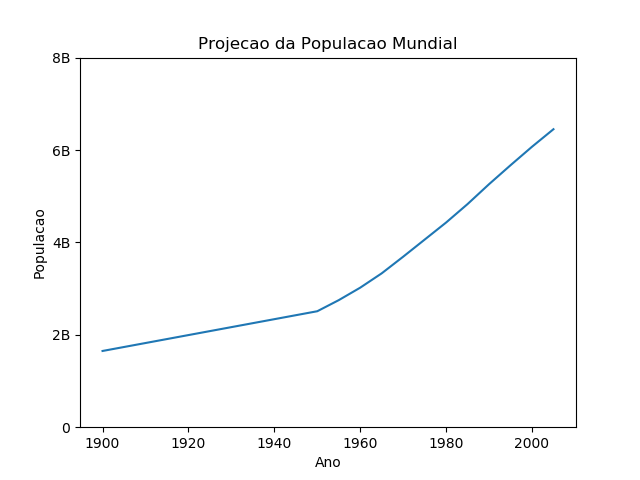
\includegraphics[scale=.35]{aula-2/figuras/matplotlib-customization-5.png}
      \end{center}
    \end{column}
  \end{columns}
\end{frame}
%
\begin{frame}[t, fragile]{Adicionando Dados Históricos}
  \begin{columns}
    \begin{column}{0.55\textwidth}
        \lstinputlisting[language=python, firstline=12]{aula-2/codigos/matplotlib/matplotlib-customization-6.py}  
    \end{column}

    \begin{column}{0.45\textwidth}
      \begin{center}
        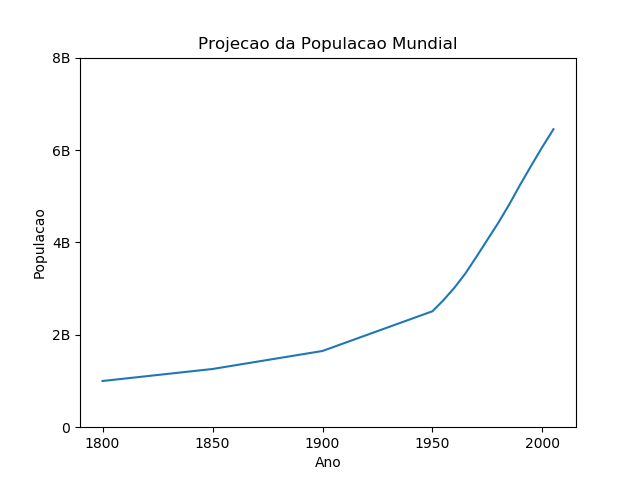
\includegraphics[scale=.35]{aula-2/figuras/matplotlib-customization-6.png}
      \end{center}
    \end{column}
  \end{columns} 
\end{frame}
%
%
\begin{frame}[t, fragile]{Antes x Depois}
  \begin{columns}
    \begin{column}{0.5\textwidth}
      \begin{figure}
        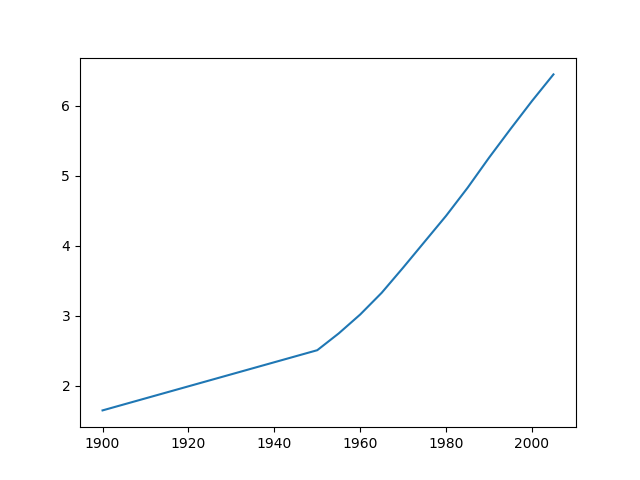
\includegraphics[scale=.35]{aula-2/figuras/matplotlib-customization-1.png}
      \end{figure}
    \end{column}

    \begin{column}{0.5\textwidth}
      \begin{figure}
        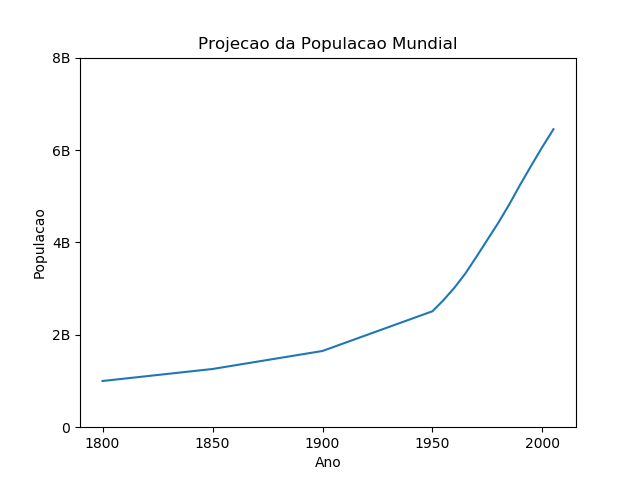
\includegraphics[scale=.35]{aula-2/figuras/matplotlib-customization-6.png}
      \end{figure}
    \end{column}
  \end{columns} 
\end{frame}


  


\end{document}

